\chapter{Contact Planの臨時更新の天体内への限定的な情報拡散の提案}
\label{chap:suggestion}
\ref{section:ContactPlanの臨時更新の課題}節で述べたとおり, 
Contact Planの臨時更新にはそれによる配送能力の向上度合いと
ネットワークへの負荷の変化によって対象を選定することが必要である. 
Contactの失敗が起きた際に全てのノードにその情報を拡散し
臨時更新を行うBezirgiannidisらの提案した既存手法に対して, 
本論文では, 情報を拡散しContact Planを更新するノードを
当該天体内のノードのみに限定し, 他天体のノードには拡散しない手法を提案する. 
本章では臨時更新におけるこれらの手法が満たすべき要件について整理し, 
その要件の観点における既存手法と提案手法の定性的な特性について述べる. 
また本論文では以降,経路や遅延について次のような表記を用いる.
\begin{table}[htbp]
    \centering
    \caption{本論文で用いる表記と意味の対応関係}
    \begin{tabular}{cc}  \hline
        本論文での表記 & 意味 \\ \hline
        R_{X \rightarrow Y \rightarrow Z} & ノードX\rightarrow ノードY \rightarrow ノードZの順の経路 \\ 
        D^{X}_{Y} & ノードXからノードYへのエンドツーエンドの遅延 \\ 
        \hline
    \end{tabular}
    \label{table:how_to_use_words}
\end{table}

\section{臨時更新の情報拡散の手法に求められる要件}
\label{section:要件定義}
\ref{section:ContactPlanの臨時更新}節で述べたように, 
Contact Planの臨時更新の目的は, 想定されたContactに失敗した場合にその
情報をDTNの他のノードに拡散しContact Planを更新することで,
DTNの各ノードが最新のトポロジーを認識し配送能力を向上することである. 
配送能力は流れているトラフィックの到達の状況によって判定されるものであり,
そのため臨時更新の手法にはまずBundleの到達率の向上と到達遅延の抑制が求められる. 

また\ref{section:ContactPlanの臨時更新の課題}節で述べたように,
Contact Planの臨時更新を行う場合, 運用するDTNへの負荷の変化を考える必要がある. 
特にDTNの運用上においては, 天体内のリンクに比べて天体間のリンクは
消費するエネルギーリソースが大きくまたContactが貴重であるため, 
この天体間のリンクの消費をできるだけ抑えることを
より優れた臨時更新手法の指標として考えることができる. 

以上より, 本論文では臨時更新手法として以下の2つを要件とする. 

\begin{center}
    \raggedright
    \begin{itemize}
        \item 要件1: 通信品質の向上 \\
                内容 : エンドツーエンドのBundleの到達率を向上させ, 到達遅延を抑制すること \\
        \item 要件2: 天体間のリンク消費抑制 \\
                内容 : 臨時更新伝達のメッセージ転送に伴う天体間リンクの消費が少ないこと
            
    \end{itemize}
\end{center}

\section{既存手法における問題点}
\label{section:既存手法における問題点}
既存手法では天体間においても臨時更新を行うため, そのメッセージにより
貴重な天体間のリンクを消費することになる.
そのため要件2において既存手法は劣ると考えられる.
既存手法のCPUPにおける更新メッセージのProtocol Data Unit(PDU)は
図\ref{figure:cpup_pdu_format}のようになっており, このPDU内で示される
Command Blockのフォーマットは図\ref{figure:command_block_format}のようになっている.
このPDUを用いて全てのノードに対して臨時更新を行う場合, そのサイズ分
天体間のリンクを消費する.

\begin{figure}[htbp]
    \centering
    \caption{既存手法におけるCPUPのPDUのフォーマット}
    \label{figure:cpup_pdu_format}
    \begin{minipage}{\textwidth}
        \centering
        \fontsize{10.5pt}{12pt}\selectfont
        参考文献\cite{Bezirgiannidis2013}Table1をもとに作成. 
        \vspace{2mm} 
    \end{minipage}
    \begin{tabular}{|c|c|c|c|}
      \hline
      Byte 0 & Byte 1 & Byte 2 & Byte 3 \\
      \hline
      \multicolumn{1}{|c|}{Version num.} & \multicolumn{3}{c|}{Number of Command Blocks (SDNV)} \\
      \hline
      Byte 4 & Byte 5 & Byte 6 & Byte 7 \\
      \hline
      \multicolumn{4}{|c|}{1\textsuperscript{st} Command Block} \\
      \hline
      \multicolumn{4}{|c|}{...} \\
      \hline
      Byte $4\times n$ & Byte $4\times n+1$ & Byte $4\times n+2$ & Byte $4\times n+3$ \\
      \hline
      \multicolumn{4}{|c|}{$n$\textsuperscript{th} Command Block} \\
      \hline
    \end{tabular}
  \end{figure}
\begin{figure}[htbp]
    \centering
    \caption{既存手法におけるCPUPのCommand Blockのフォーマット}
    \label{figure:command_block_format}
    \begin{minipage}{\textwidth}
        \centering
        \fontsize{10.5pt}{12pt}\selectfont
        参考文献\cite{Bezirgiannidis2013}Table2をもとに作成. 
        \vspace{2mm} 
    \end{minipage}
    \begin{tabular}{|c|c|c|c|}
      \hline
      Byte 0 & Byte 1 & Byte 2 & Byte 3 \\
      \hline
      \multicolumn{2}{|c|}{Creation Timestamp (SDNV)} & \multicolumn{2}{c|}{Command Expiry (SDNV)} \\
      \hline
      Byte 4 & Byte 5 & Byte 6 & Byte 7 \\
      \hline
      \multicolumn{3}{|c|}{Command Originator (SDNV)} & Command Type \\
      \hline
      Byte 8 & Byte 9 & ... & Byte $n$ \\
      \hline
      \multicolumn{2}{|c|}{Command Parameter 1 (SDNV)} & \multicolumn{1}{c|}{...} & Comm. Param. $k$ (SDNV) \\
      \hline
    \end{tabular}
\end{figure}

\section{本研究の提案手法}
\label{section:要件1における既存手法と提案手法の比較}
\ref{section:既存手法における問題点}節で述べたように, 既存の手法ではDTNのすべてのノードに情報を拡散し
Contact Planを更新するため天体間リンクが消費されることを問題である.   
本研究ではこれに対し, 対象を当該天体内のノードのみに限定することで, 天体間でのメッセージの転送を行わない手法を提案する.

一方要件1については, 既存手法も提案手法もどちらもDTNの各ノードに最新の
トポロジーを認識させることが目的であるため,
どちらの手法も用いず更新を行わない場合に比べると
配達率の増加と遅延の抑制に寄与することが期待される.
しかし既存手法は提案手法よりもより多くのノードに更新情報を拡散するため,
より到達率の向上と遅延の抑制への寄与する, 
すなわち要件1において提案手法よりも基本的には優れていると考えられる. 
ただし既存手法における拡散はその更新メッセージを天体間の遅延を超えて
届ける必要があり, それ以前においては提案手法と
同様に天体内のノードにのみ拡散されるため, 
要件1について提案手法は既存手法には劣るものの, その差異は小さいことが予想できる. 

以下では具体的な例として図\ref{fig:experimentation_topology}のトポロジーを用いて
要件1における既存手法と提案手法の効果について考える.

\begin{figure}[tbh]
    \centering
    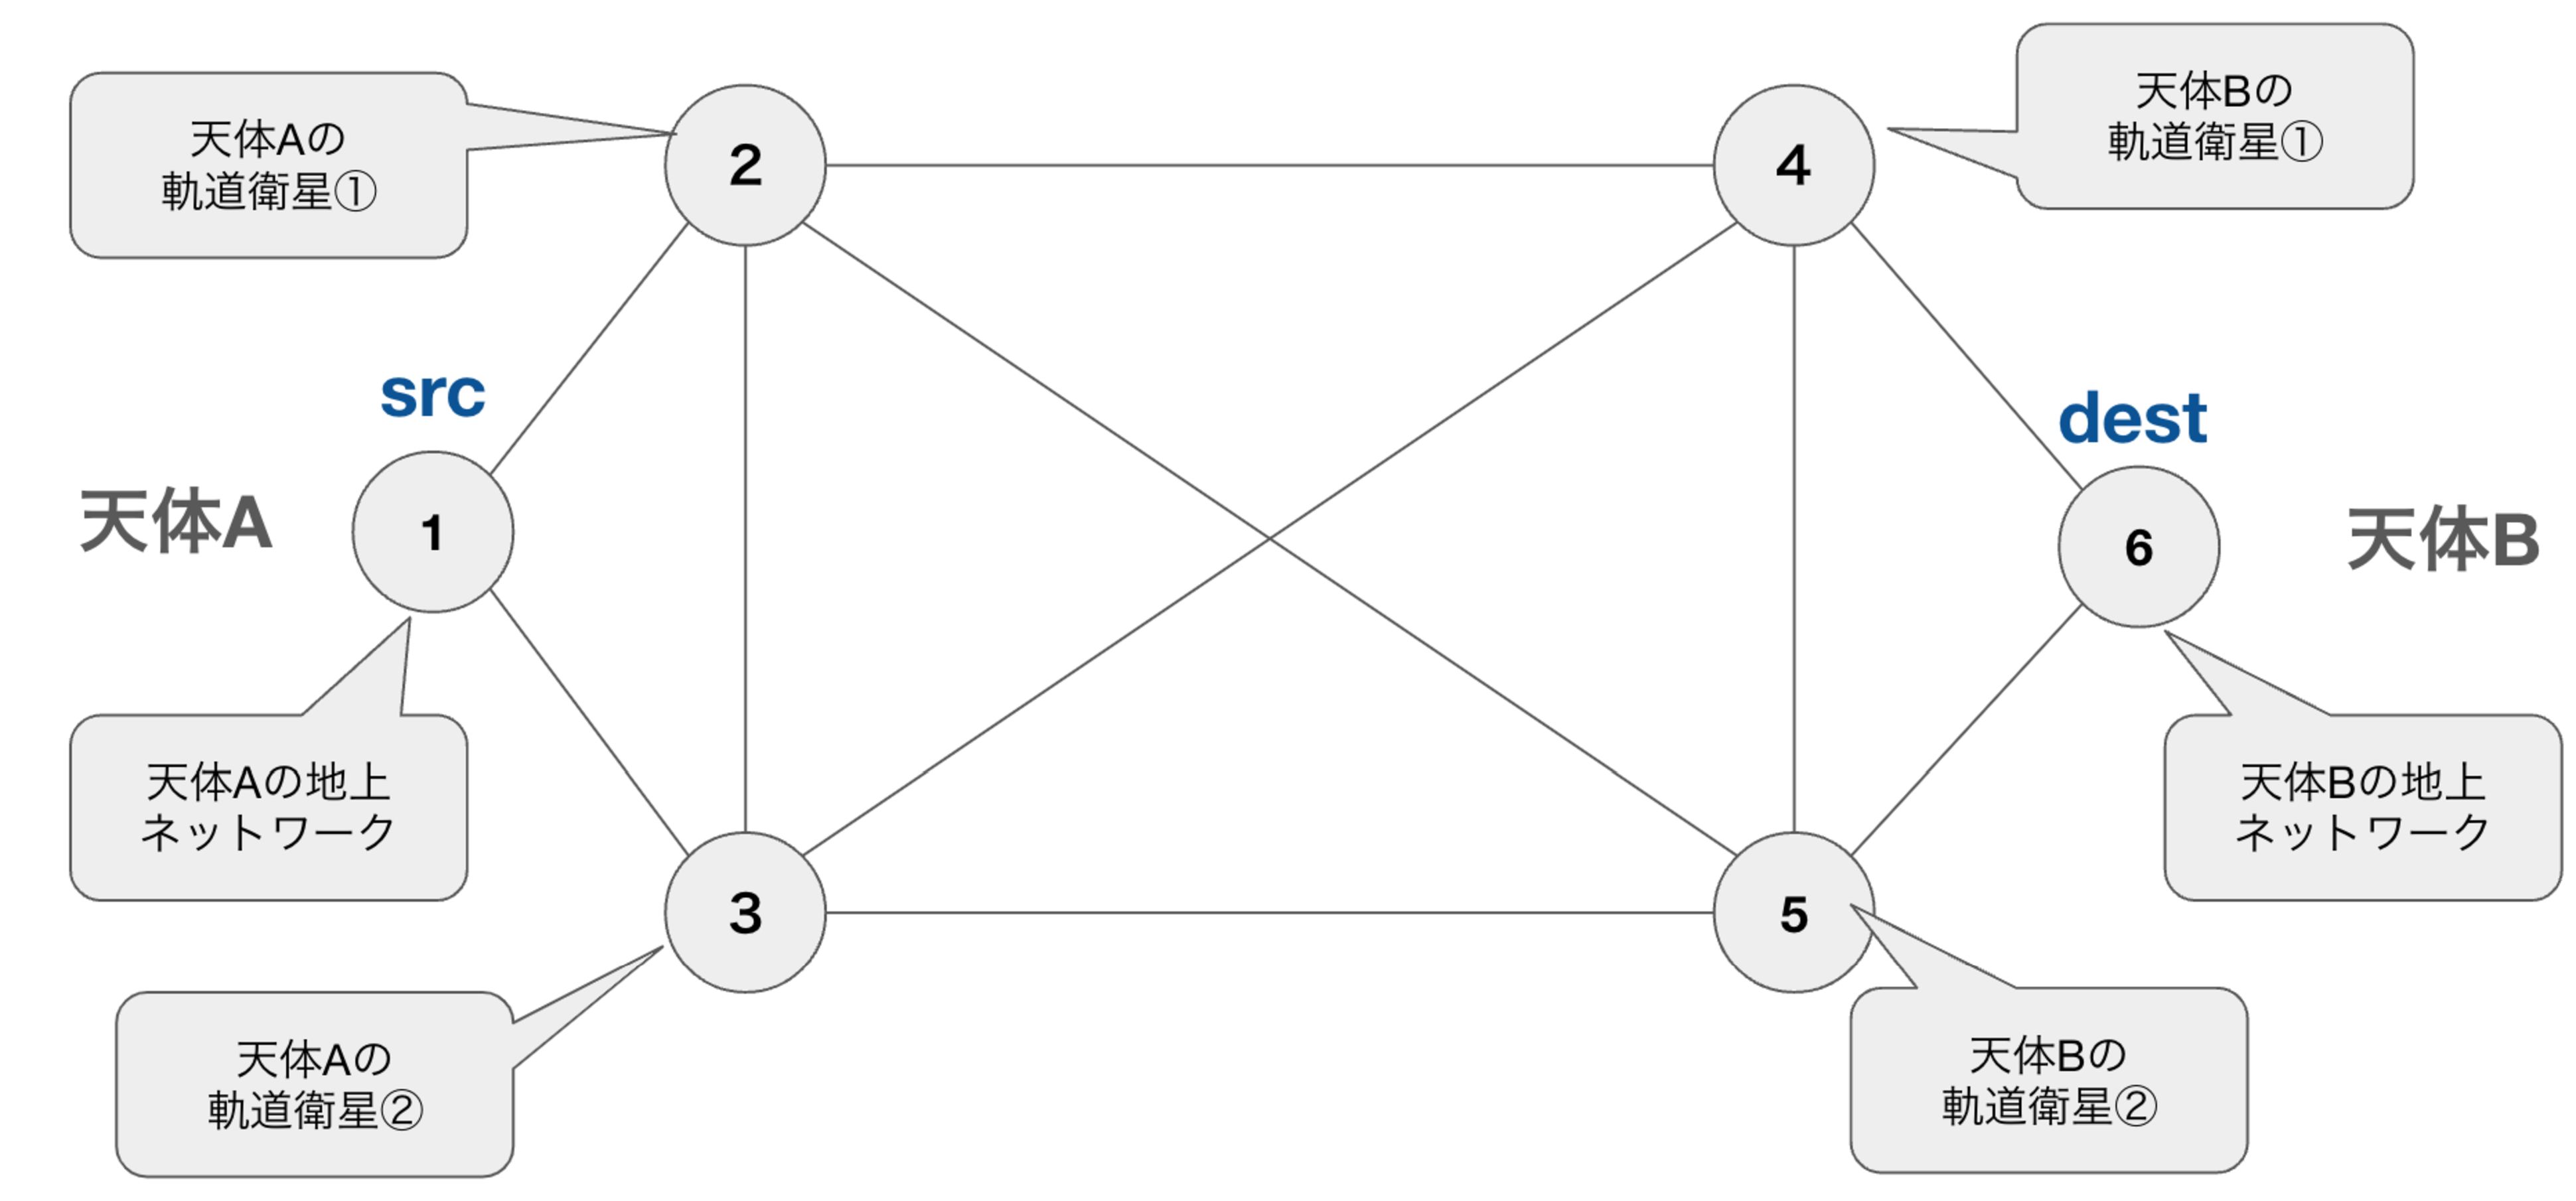
\includegraphics[width=0.7\textheight]{img/thesis_Sample_topology.pdf}
    \caption{本実験で用いるトポロジー}
    \label{fig:experimentation_topology}
    \begin{minipage}{\textwidth}
        \centering
        \vspace{3mm}
        \fontsize{10.5pt}{12pt}\selectfont
        ノード1は天体Aの地上DTNネットワークを代表したノード, ノード2とノード3は
        天体Aの軌道上に存在する宇宙のDTNノード, ノード4とノード5は
        天体Bの軌道上に存在する宇宙のDTNノード, 
        ノード6は天体Bの地上DTNネットワークを代表したノードを示す. 
    \end{minipage}
\end{figure}

ノード1から3は天体A, ノード4から6はそれぞれ天体Bに属するDTNノードであり, 
ノード1と6はそれぞれの地表DTNのノード, ノード2から5はそれぞれの天体の軌道上にある
宇宙のDTNノードである. 
このトポロジーにおいて, 図\ref{fig:example_of_routechange}のように
今ベストパスが R_{1 \rightarrow 2 \rightarrow 4 \rightarrow 6}(経路1)であるとし, 仮に
ノード4から6のContactが何らかの理由で失敗した場合に, 
ベストパスはR_{1 \rightarrow 2 \rightarrow 5 \rightarrow 6}の経路(経路2)となり, 
ただしこれよりは最適経路ではないものの
R_{1 \rightarrow 2 \rightarrow 4 \rightarrow 5 \rightarrow 6}(の経路(経路3)でもBundleの配送が可能であるとする.

\begin{figure}[tbh]
    \centering
    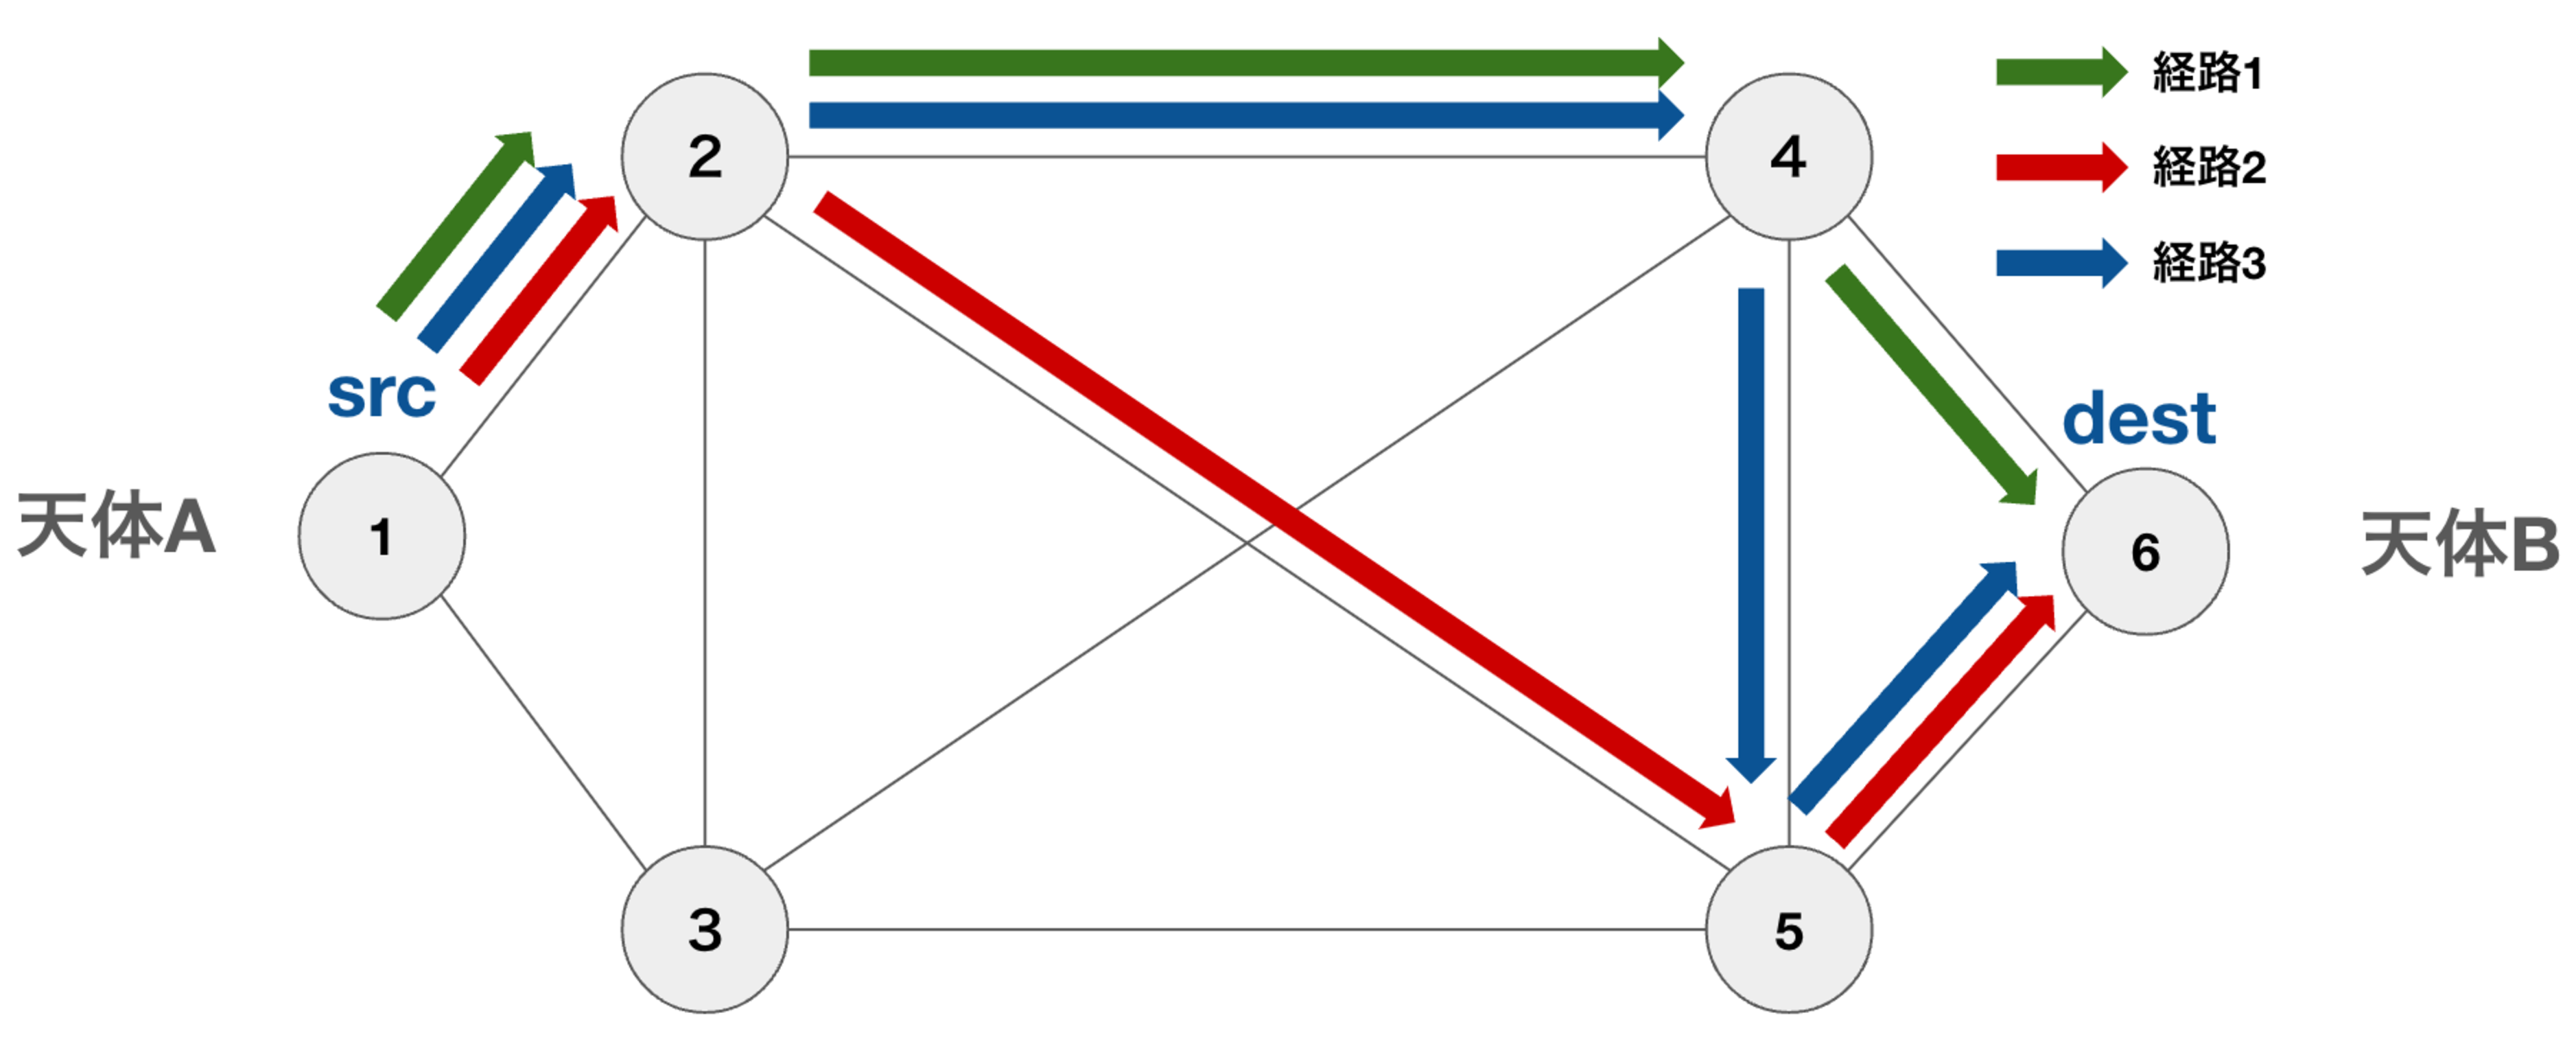
\includegraphics[width=0.7\textheight]{img/example_of_routechange.pdf}
    \caption{Contact失敗時に既存手法と提案手法において選択される代替経路の例}
    \label{fig:example_of_routechange}
\end{figure}

既存手法も提案手法も用いず更新を行わない場合, どのノードもそのContactの失敗を知らないため
すべてのノードはベストパスが経路1のままと認識し, ノード4においてノード6へのBundleの配送を試み続ける.
TTLの期限切れまでそれを試み続けるため, 図\ref{fig:example_of_delaychange}中の黒線のように, 
障害発生中はBundleが到着せず, そのContactの復旧が起きた場合, もしくは
最適経路が当該Contactを使用しない経路に切り替わった時にBundleの送信が成功するようになる. 

既存手法では, その情報をノード4を起点に発信し, その情報を受け取ったノードは順次Contact Planから
当該Contactを削除し, Contact Planを更新する. これにより, 失敗発生直後よりノード4は代替経路となる経路3を
利用することが可能になり, 経路1と比較して到達遅延は増加するものの, Bundleの送信には成功する. さらにこの場合, 
天体間遅延を超えてこの情報が天体Aのノード1・2・3に配信されると, 
ノード2は経路2が最適経路と認識することができるようになり, 経路3よりも配送遅延を低下させることができる. 
そのため既存手法における障害発生時の到達遅延の推移は図\ref{fig:example_of_delaychange}中の紫線のようになる. 

提案手法では, 当初は既存手法同様経路3をすぐに利用できるようになるが, 
天体間には更新情報を伝搬しないため経路2が利用されることはなく, 
そのため提案手法における障害発生時の到達遅延の推移は図\ref{fig:example_of_delaychange}中の黄線のようになる. 

\begin{figure}[tbh]
    \centering
    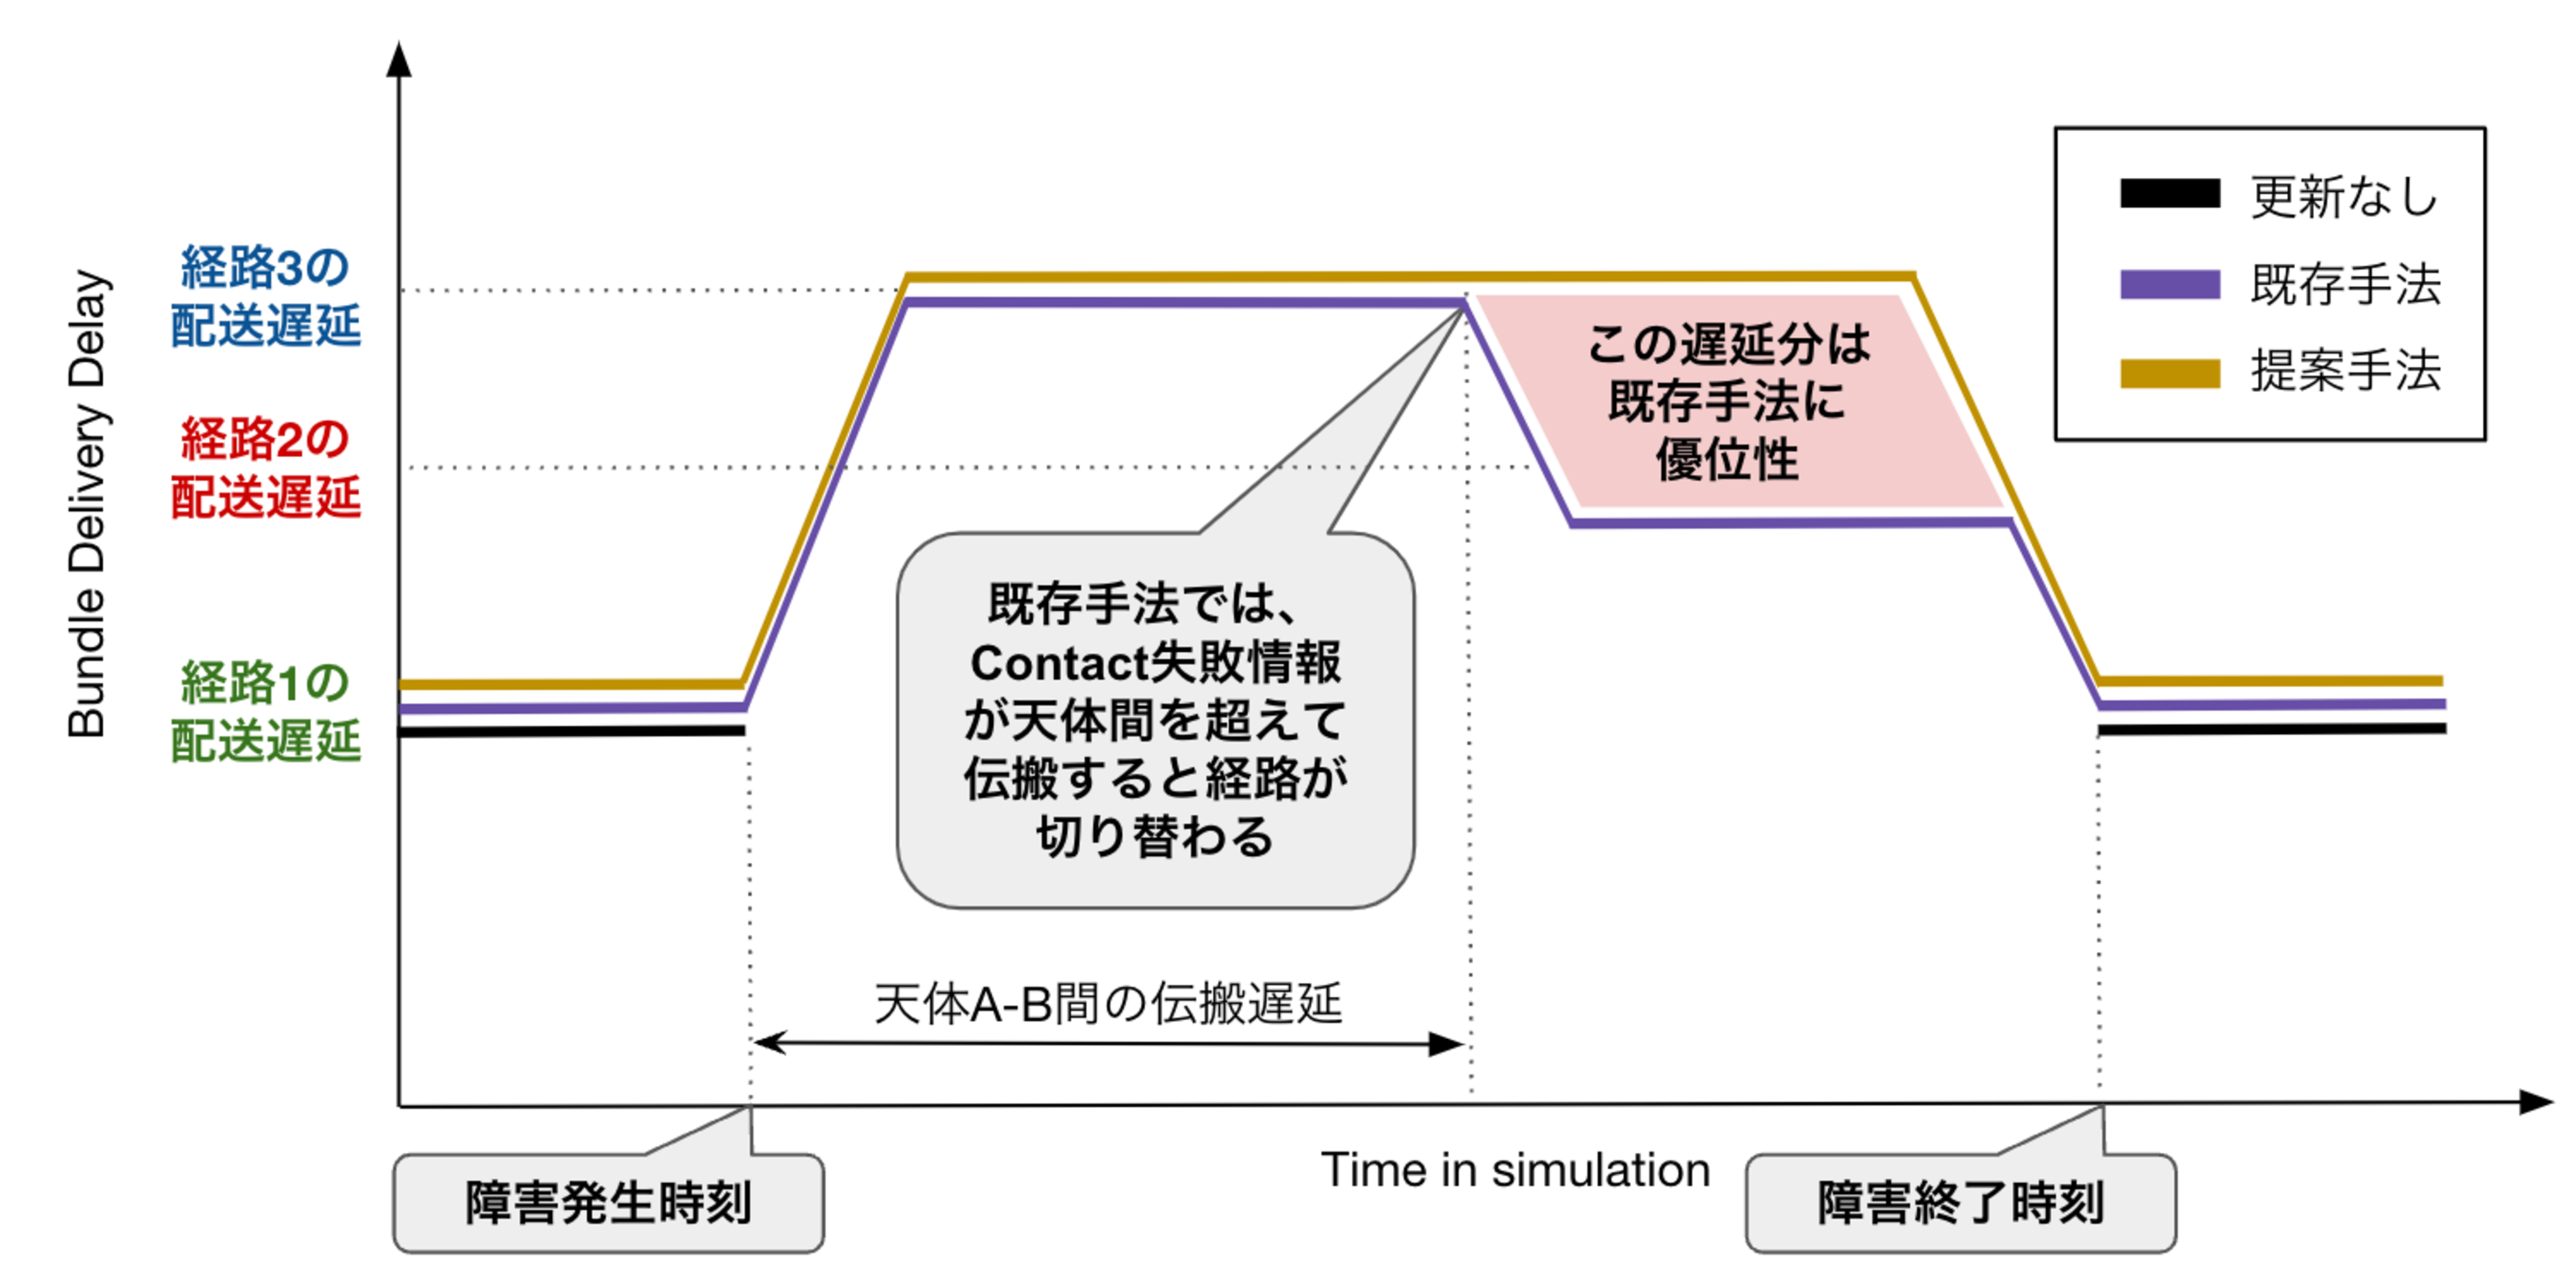
\includegraphics[width=0.7\textheight]{img/example_of_delaychange.pdf}
    \caption{Contact失敗時の配送遅延変化の予想}
    \label{fig:example_of_delaychange}
\end{figure}

既存手法と提案手法の差はすなわち経路2と経路3の遅延の差(図\ref{fig:example_of_delaychange}中の赤い部分)である.
しかしこれはノード2からノード4の遅延とノード2からノード5の遅延の差, 
すなわち天体Bの2つの衛星の天体Aの衛星との距離の差によるものである. 
これは経路全体の長さに比べると比較的短いものであると考えられ, 既存手法で途中から経路2を利用できることの
利点は限定的である. そのため, 配送遅延の低下という点に置いて当然提案手法の有効性はあるものの, 
提案手法も既存手法に近しい有効性があると予想される.  
  